\chapter{Interface utilisateur}
\section{Le besoin}
L'interface utilisateur est essentielle dans notre projet.
Il faut que le programme soit simple d'utilisation.
Cela passe par une interface graphique facile d'utilisation. De même, il faut que l'affichage du procédé de résolution soit clair.
Nous avons fait le choix d'afficher un cube en 3D.

\section{Interface Homme Machine}
\subsection{Les classes utilisées pour l'IHM}
L’interface utilisateur à été réalisée à partir de la bibliothèque \textit{swing}. Nous l’avons produite suivant le diagramme UML de classes suivant :

 \begin{figure}[h]
 \begin{center}
       \makebox[\textwidth]{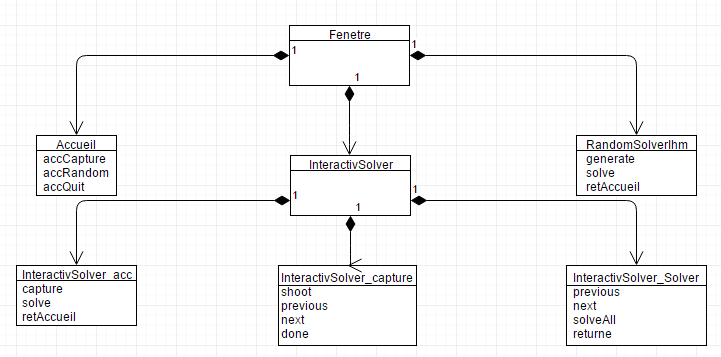
\includegraphics[width=.8\paperwidth]{diagrammes/classes_ihm.png}}
 \end{center}
     \caption{Diagramme des classes de l'IHM}
 \end{figure}


La classe principale, \textit{Fenetre}, va créer la fenêtre de notre programme. Elle contient le main du projet.
Elle agit ici comme un gestionnaire de scène d’où sa composition en 3 classes.

Ainsi, on a 3 scènes dans le projet… du moins 3 scènes principales, \textit{InteractivSolver} étant lui même un gestionnaire de scènes.

\subsection{L'accueil}
Lorsqu’on lance notre programme, nous arrivons sur la scène \textit{Accueil}. Elle est composée, comme on peut le voir sur le diagramme, de 3 boutons :

\textbf{//expliciter les boutons et faire des screen shot de l’interface en rendu}
\begin{itemize}
    \item Bouton accRandom 
    ⇒ passage de la scène \textit{Accueil} à la scène \textit{RandomSolverIhm}
    \textbf{⇒ Screenshot de la fenetre}

    \item Bouton generate : génère un RubiksCube aléatoire
        ⇒ explication de scramble dans OpenGLRenderer

    \item Bouton solve : résout le RubiksCube ainsi généré sans détailler les étapes
        ⇒ explication Solve dans OpenGLRenderer

    \item Bouton ret\textit{Accueil} : passe de la scène actuelle à la scène \textit{Accueil}

    \item Bouton accQuit : ferme le programme

    \item Bouton accCapture : Passe de la scène \textit{Accueil} au gestionnaire de scène \textit{InteractivSolver}

\end{itemize}

\subsection{Le gestionnaire de scène}
\underline{Gestionnaire de scène \textit{InteractivSolver}}
⇒ affiche en premier lieu \textit{InteractivSolver}
\begin{itemize}
    \item Bouton capture : passe de la sène accueil à la scène \textit{InteractivSolver\_capture}
    \item Bouton solve : passe de la scène accueil à la scène \textit{InteractivSolver\_solver}
    \item Bouton ret\textit{Accueil} : passe du gestionnaire de scène \textit{InteractivSolver} à la scène \textit{Accueil}
\end{itemize}

\subsection{L'interface de capture}
\underline{InteractivSolver\_capture :}
\begin{itemize}
    \item Bouton Shoot : prend en capture la webcam, analyse les couleurs en certains point et affiche la face ainsi capturé à l’indice correspondant (cf partie sur image processing pour détail)
    \item Bouton previous : passe à la capture de la face précédente
    \item Bouton next : passe à la capture de la face suivante
    \item Bouton done : la capture est terminé, passe de la scène \textit{InteractivSovler\_capture} à \textit{InteractivSolver\_acc}
\end{itemize}

\subsection{L'interface de résolution}
\underline{InteractivSolver\_solver :}
\begin{itemize}
    \item Bouton previous : Revient au mouvement précedent
    \item Bouton next : passe au mouvement suivant :
    \item SolveAll : termine la solution seul.
    \item Return : passe de la scène \textit{InteractivSolver\_solver} à \textit{InteractivSolver\_accueil}
\end{itemize}

\section{L'affichage en 3D - OpenGL}

Cette bibliothèque est utilisé comme moteur graphique 3D pour dessiner le cube.

\subsection{Fonctionnement général d'OpenGL}
OpenGL fonctionne de la façon suivante :
	Une scène est créée par le biais de l’objet GLU et GL2.
	Quatre méthodes sont alors redéfinies.

\begin{itemize}
    \item \underline{Init} : comme son nom l’indique, on initialise notre scène avec différentes méthodes de la bibliothèque. On lui applique également un fond noir pour un soucis de visibilité.

    \item \underline{Display} : C’est la méthode la plus importante d’OpenGL. Il s’agit d’une boucle infinie qui va actualiser notre rendu. Cette méthode définie d’une certaine façon notre “framerate”.
C’est sur cette particularité qu’il va falloir jouer et qui peut s’avérer être complexe dès lors que l’on veut faire des animations. Nous reviendrons en détails sur sa construction à la fin de cette partie.

\item \underline{Dispose}  : Nous n’en avons pas besoin ici mais elle doit être réécrite pour que le rendu fonctionne.
Reshape : Permet de changer la taille du rendu. Cette méthode a été redéfinie même si finalement nous imposons une taille fixe dans l’interface final.

\end{itemize}

\subsection{Transformer le cube}
Maintenant que nous avons notre socle de base de notre moteur graphique, il faut dessiner le cube.

La principale difficulté a été de traduire les informations que la classe RubiksCube me fournissait. En effet, lorsque nous instancions un \textit{RubiksCube}, ce dernier possède une table de permutation qui permet la résolution. Le cube est alors défini par facettes (entité qui représente une couleur d’une face du cube). Hors, il était plus simple pour le rendu 3D de dessiner des petits cube (vis à vis de l’animation).

On a alors créé la classe \textit{Cube} dont le constructeur prend en argument 6 couleurs de l’enum Color ainsi que 3 entiers correspondant à la position d’un cube avec une norme arbitraire choisie par nos soins.

La méthode \textit{setCube}, bien que fastidieuse, nous permet donc d’avoir une liste des différents cubes que compose le RubiksCube. Comme un cube ne possède qu’au plus 3 faces visibles, nous plaçons les autres faces, interne au RubiksCube, en noir.

\subsection{Dessiner le cube}
\subsubsection{Affichage du cube}
On peut donc dès à présent dessiner notre RubiksCube. C’est pourquoi nous avons fait la méthode \textit{drawRubikscube} 
\textbf{(mettre ici la méthode (40 lignes ~)}

\begin{enumerate}
    \item setCube
    \item 3 imbrications de boucle for pour parcourir toutes nos coordonnées
    \item PushMatrix pour pouvoir dessiner sur notre scène
    \item Le pointeur revient au centre
    \item Les 3 rotate sont là pour l’animation, nous verront cela plus tard
    \item On sélectionne le cube à dessiner à la position [x,y,z]
    \item La succession de if est là pour déplacer nos cubes d’un petit écart pour donner les petites bandes noires entre chaque petit cube
    \item On dessine le cube par la méthode drawCube dont voici un extrait.
    \item On PopMatrix pour indiquer que notre dessin est terminé.
\end{enumerate}

Cette méthode est donc appelée dans \underline{Display}, ce qui signifie qu’elle est appelée en boucle par notre scène de rendu.

\subsubsection{Animation du cube}
Ainsi, pour faire une animation, on doit faire une méthode qui, pour une rotation donnée, sélectionne l’axe de rotation, les cubes à faire tourner et le sens de rotation (trigonométrique ou horaire)

L’objectif est donc, de faire tourner les cubes frame par frame, par incrémentation de l’angle dans drawRubiksCube que l’on vient de voir pour donner une sensation d’animation. C’est ce que réalisait les 3 glRotatef ci-dessus :  \textbf{(remettre le bout de code)}

\textbf{//Dessiner un rubik’s cube avec les 3 axes et coordonnée pour expliquer les trois float[3] dans Rotate sur un exemple.}

\paragraph{Comment cette rotation a été faite ?}
3 méthodes :
\begin{itemize}
    \item isRotating : pour effectuer une seule rotation à la fois. rotateX, rotateY,rotateZ égaux à -1 si on ne tourne pas sur l’axe correspondant.
    \item rotate (int face, Axis axis, boolean clock) :
face va être un entier qui sera égale à soit 0, soit 2 et nous permettra de sélectionner la face à tourner selon l’axe axis. Ainsi, si l’on veut tourner la première face qui est centrée sur l’axe X dans le sens horaire, on aura rotate(int 0, Axis.X, boolean clock) qui affectera à rotateX la valeur 0 et rotationSpeed,qui est la valeur d’incrémentation de l’angle que l’on effectue à chaque frame, qui est fixe en valeur absolue mais qui est soit positif ou négatif selon le sens de rotation d’où l’opérateur ternaire qui est en fin de méthode.
    \item Il reste alors la méthode principale, updateAngles qui est, rappelez vous, celle qui était appelé en première dans Display().
\end{itemize}

\paragraph{Explications}
Supposons que l’on soit à un instant t quelconque et reprenons notre précédent exemple (rotate(0,Axis.X,true) ).

updateAngles() est appelée. Comme une seule rotation est faite à la fois, seul une des trois variables parmis rotateX,rotateY et rotateZ est positive ou nulle.

Dans un premier temps, et pour des raisons de clareté, on définit une direction de l’enum Direction par l’opérateur ternaire \textbf{(placer ici le code )}. Cette ligne est tout à fait supprimable mais elle rend le code plus lisible pour la suite.
\textbf{// 	code OpenGLRenderer ligne 322 à 365}

On rentre alors dans l’une des trois conditions. Pour notre exemple, c’est rotateX = 0

Souvenez vous des glRotate dans drawRubiksCube, on effectuait une rotation d’angle coloneAnglesX[x] pour l’axe X (resp. axe Y, axe Z). Comme l’on veut tourner la face 0 de l’axe X, on va donc incrémenter la valeur de cette angles jusqu’à une valeur limite qu’est 90°.

Ainsi, à une frame f quelconque, la face en question sera tourné d’angle coloneAnglesX[x].

On incrémente alors coloneAnglesX[rotateX =0] de la valeur de rotation Speed.

On vérifie ensuite que l’angle est égale à 90° (Note : on suppose ici que l’angle rotationSpeed est un diviseur de 90).

Si ce n’est pas le cas, on passe à la suite et la valeur sera incrémenté au prochain appel de Display (donc de updateAngles)

Supposons maintenant que coloneAnglesX[0] = 90.

On la définit alors = 0 pour réinitialiser la matrice d’angles de rotation.

puis il faut maintenant effectuer la rotation de l’objet RubiksCube pour qu’il n’y ait aucune différence entre la configuration dans le rendu et celle dans RubiksCube.

\textbf{//mettre ici les 4 if}

puis comme la rotation est terminée, on peut remettre rotateX (resp. rotateY, rotateZ)  à la valeur -1.

Les dernières méthodes sont utile à d’autres classes, notamment dans l’interface et seront donc explicité plus tard.

\paragraph{Résumé}
Je vous propose alors de résumer tout ce que l’on vient de préciser par parcourir une itération de Display()
updatesAngles : On vient d’expliquer sa fonction qu’est de mettre à jours les angles d’une frame à l’autre.
\begin{itemize}
    \item on récupère l’objet GL2 qui constitue notre scène

    \item glClear : On vide différents buffer pour éviter tout problème de superposition de tracé dans notre rendu final.

    \item glLoadIdentity : réinitialise la matrice que l’on a dessiné à la frame précédente (cf. pushMatrix dans drawRubiksCube)

    \item gluLookAt(0f,0f,12f,0f,0f,0f,0f,1f,0f) : Place le point de vue à la position [0,0,12], regardant vers [0,0,0] selon l’axe [0,1,0] (ici l’axe Y). Les valeurs sont arbitraire et empirique

    \item glRotate(alphaX (resp. alphaY,alphaZ)). Permet de tourner l’intégralité de la scène selon les trois axes et permet donc de tourner autour du RubiksCube. Ces rotations sont réalisé par appuie sur les touches fléchées du clavier dans les classes de l’interface contenant un OpenGLRenderer.

    \item drawRubiksCube : dessiner le RubiksCube avec les différents paramètre de rotation.
\end{itemize}















